\subsection{Réseaux Pair a Pair}
Comment proposer un service de co-voiturage localisé, personnalisé et adapté a chaque catégorie?\\
Pour répondre a ces questions, on se propose de créer 2 réseaux P2P, un pour chaque catégorie, permettant de garantir la confidentialité des données entre les réseaux. Ces deux réseaux correspondent a deux versions d'un logiciel que nous proposons sous forme d'application web, ou smartphone: myTransport \\

~~~ 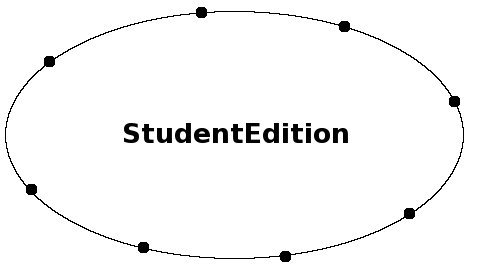
\includegraphics[scale=0.35]{img/schema/StudentEdition} ~~~~~~~~~~ 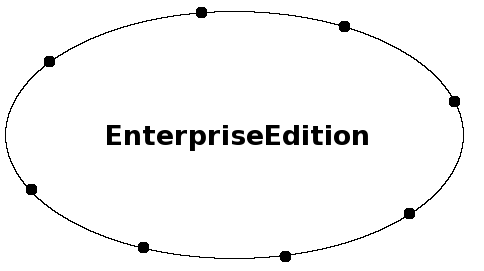
\includegraphics[scale=0.35]{img/schema/EnterpriseEdition} \\

L'idée du réseaux P2P est né de plusieurs constats: 
\begin{itemize}
\item Un réseau P2P est autonome, et ne nécessite pas de mise en place ou de déploiement complexe dans une entreprise pour fonctionner. Aucun serveur, aucune machine n'est sollicitée. Aucune démarche administrative a effectuer, c'est a dire pas de barrière au lancement du projet.
\item De plus, les réseaux P2P sont tolérant au pannes, ils ne sont pas dépendant du bon fonctionnement d'un seul serveur.
\item L'arrivée sur le marché des smart-phones et autres tabletPC laissent imaginer beaucoup d'applications et d'évolutions pour un simple réseau de co-voiturage (géolocalisation en temps réel, RFID détection automatique du statu d'une personne, voir 5eme partie...).
La structure de donnée que nous choisissons ici est celle des DHTs. Cette structure permet d'associer a une clef, n'importe quelles valeurs. Le protocole de routage utilisé dans cette exemple est Chord. Ce protocole complètement scalable garanti l'exhaustivité des données. \\
\end{itemize}

\clearpage

\subsection{Exemple de fonctionnement: }
Soit une la zone géographique délimitée par les villes de: Nice, Cagnes-sur-Mer, Antibes, Sophia-Antipolis. \\

~~~~~~~~~~~~~~~~~~~~ 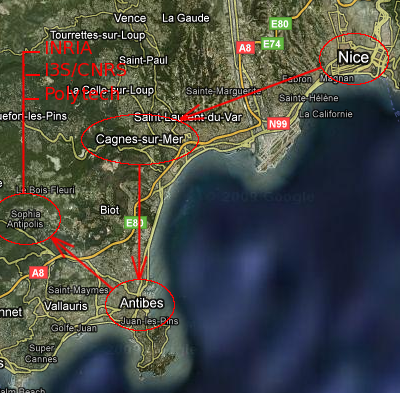
\includegraphics[scale=0.7]{img/screenshot/geolock2}\\

Un ingénieur expert souhaite, pour réduire le coup de son trajet journalier, faire du co-voiturage. Il décide alors de publier une proposition de covoiturage dans son réseau P2P:\\ 

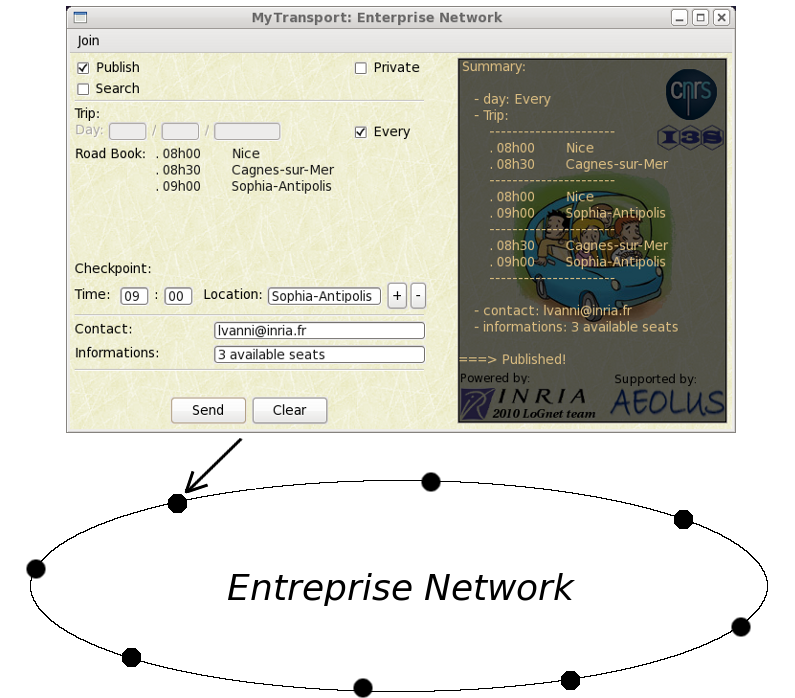
\includegraphics[scale=0.6]{img/screenshot/enterprisePub}\\

Les différents champs que nous voyons ici représentent plusieurs valeurs associées a plusieurs clefs, explications:\\
Tout d'abord, la partie Trip:
\begin{itemize}
\item Le premier champ concerne la date à laquelle le trajet va être effectué: L'utilisateur peut soit saisir la date soit cocher la checkBox "Every" qui permet de préciser qu'il s'agit d'un trajet journalier.
\item La deuxième partie (Road Book), permet d'enregistrer l'itinéraire prévu:
			\begin{itemize}
			\item 08h00 Nice
			\item 08h30 Cagnes-sur-Mer
			\item 09h00 Sophia-Antipolis
			\end{itemize}
\end{itemize}
Cette partie permet de créer toutes les clefs correspondant à tous les itinéraires possible:
\begin{itemize}
\item Clef 1 : Nice 08h00 | Cagnes-sur-Mer 08h30 | Every days
\item Clef 2 : Nice 08h00 | Sophia-Antipolis 09h00 | Every days
\item Clef 3 : Cagnes-sur-Mer 08h30 | Sophia-Antipolis 09h00 |  | Every days \\ ~ \\
\end{itemize}

La deuxième partie, constitue la valeur associée a chacune de ces clefs. Cette valeur est la concaténation des informations:
\begin{itemize}
\item Contact = Nom de la personne concernée, email, téléphone, ...
\item Informations = Toutes informations utiles (Nombre de place, type de voiture, ...) \\
\end{itemize}

Cette proposition de co-voiturage va donc être visible de tous les membres non étudiants des trois centres de recherches. Un utilisateur cherchant donc une proposition de co-voiturage entre Nice et Sophia-Antipolis obtiendra:\\

~ 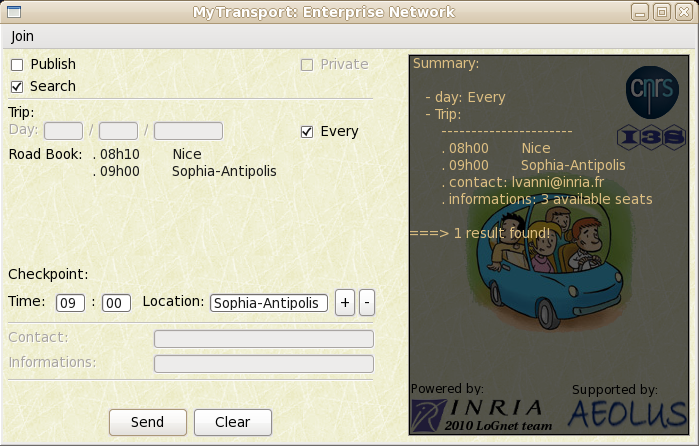
\includegraphics[scale=0.55]{img/screenshot/NiceSophiaSub}\\

Un autre aspect de cette application, est qu'il possible de réunir plusieurs itinéraires déjà publiés pour les combiner et en faire d'autres pour répondre à plus de demandes:

~ 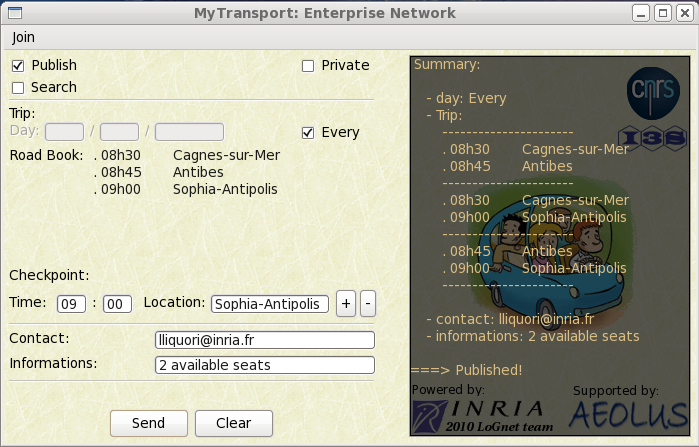
\includegraphics[scale=0.55]{img/screenshot/CagnesAntibesSophiaPub}\\

Ici on peut voir un utilisateur qui publie un nouvel itinéraire avec cette fois-ci Antibes en point de passage.\\

Supposons maintenant qu'un autre utilisateur souhaite faire le trajet:
\begin{itemize}
\item 08h00 Nice
\item 08h30 Cagnes-sur-Mer
\item 08h45 Antibes \\
\end{itemize}

~ 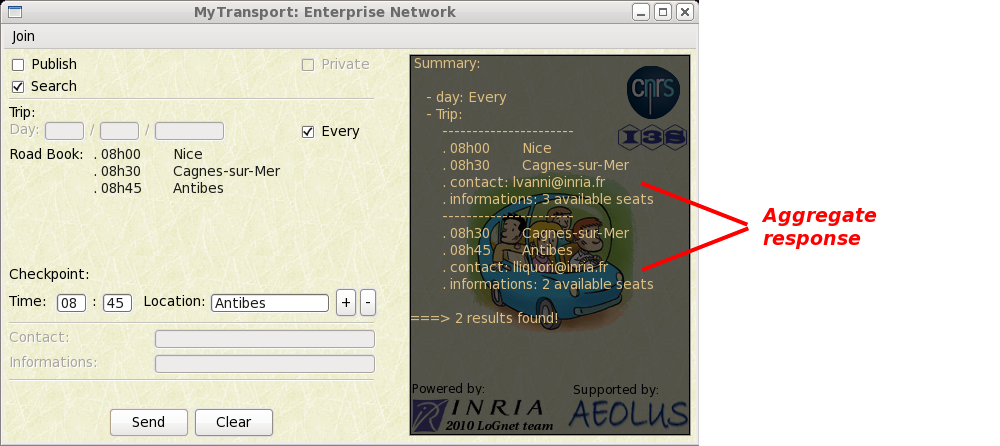
\includegraphics[scale=0.50]{img/screenshot/NiceCagnesAntibesSub}\\

Nous voyons ici que la requête issue de la demande à permis de générer un résultat composer de plusieurs propositions de covoiturage différentes.\\ ~ \\

L'ingénieur expert peut ainsi profiter du système de co-voiturage avec ces collègues des différents centres de recherches de Sophia-Antipolis. Malgré cela, il reste encore des places disponibles dans sa voiture pour son trajet quotidien. Pour optimiser encore plus l'utilisation de sa voiture, il souhaiterai maintenant partager ses informations avec les étudiants qui disposent de leur propre réseaux de co-voiturage (ici identique au niveau du fonctionnement).\\

~ 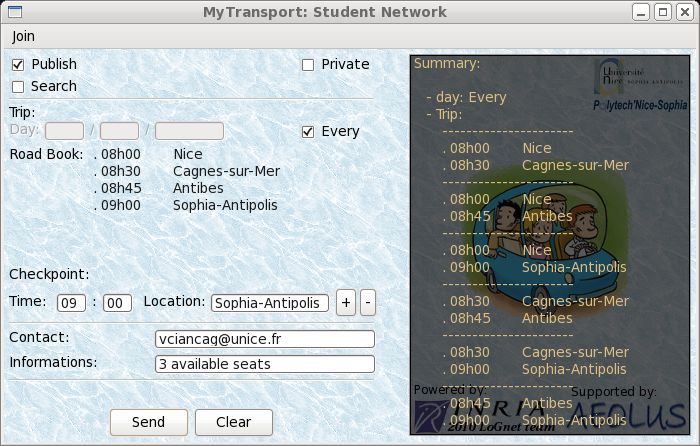
\includegraphics[scale=0.55]{img/screenshot/NiceCagnesAbtibesSophiaPub_studentNetwork}\\

Pour cela on une checkBox "private" , qui permet de préciser si l'on souhaite rendre ces informations publique (c'est a dire qu'elles soit visible depuis d'autres réseaux) ou pas.
Cette seule indication ne suffit pas a diffuser l'information en dehors du réseaux, les deux réseaux de notre exemple étant hétérogènes et a priori non collaboratifs. Pour y parvenir nous allons maintenant introduire le concept de Synapse, dont le but est d'inter-connecter ce genre de réseaux.

